% VerdeAI decision-derivation approach — state_compare (old) vs slot_fill (new).
% Standalone: compiles alone to one cropped page.
\documentclass[tikz, border=6mm]{standalone}
\usetikzlibrary{shapes.geometric, arrows.meta, positioning, calc, decorations.pathreplacing}

\definecolor{inkcolor}{HTML}{17241B}
\definecolor{mutedtext}{HTML}{4D5D4F}
\definecolor{iofill}{HTML}{B7C6DA}
\definecolor{processfill}{HTML}{BFD3BC}
\definecolor{aifill}{HTML}{CBB9D6}
\definecolor{decisionfill}{HTML}{E6D3A3}
\definecolor{oldfill}{HTML}{E3B7B0}
\definecolor{newfill}{HTML}{9FC2B2}

\begin{document}
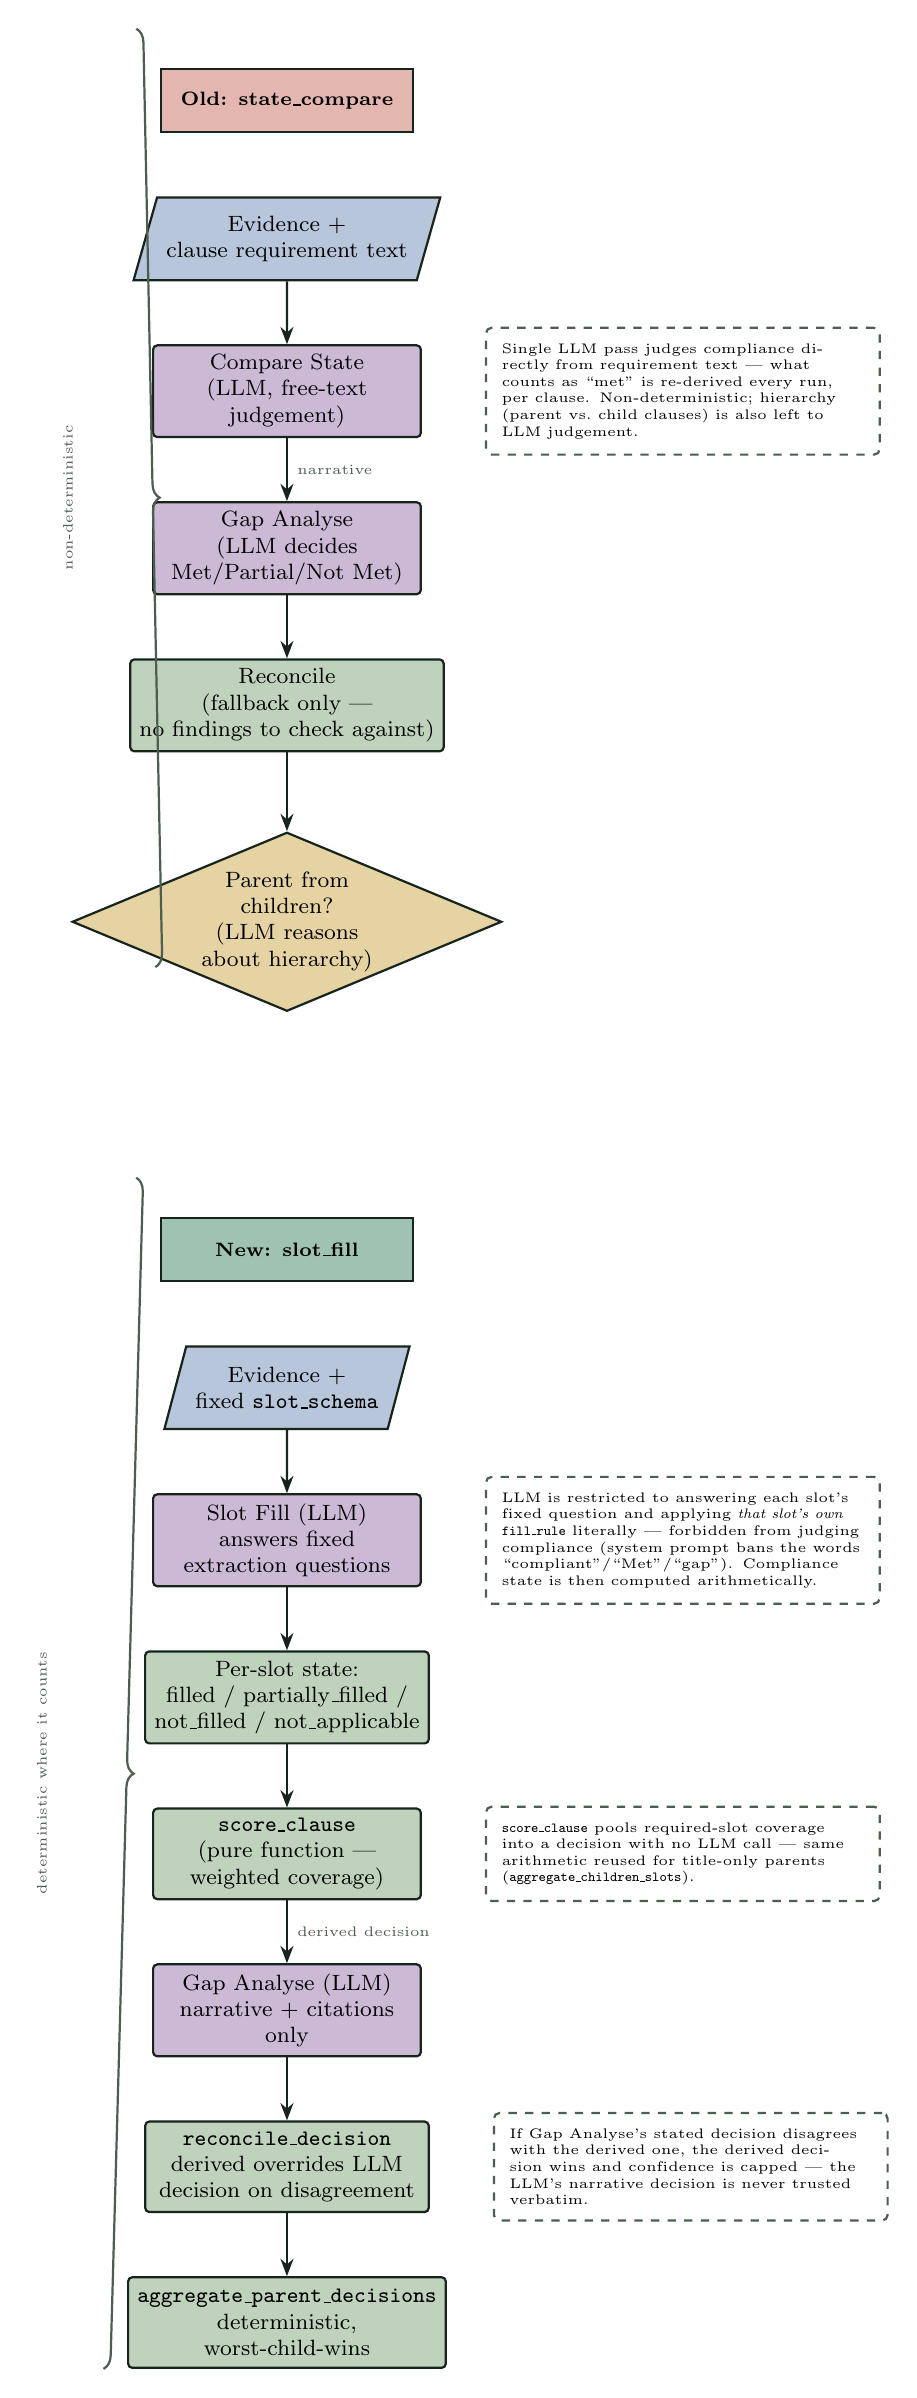
\begin{tikzpicture}[
  >=Stealth, every node/.style={font=\footnotesize},
  node distance=6mm and 6mm, align=center, thick,
]

\tikzset{
  io/.style={trapezium, trapezium left angle=70, trapezium right angle=110,
    trapezium stretches=true, draw=inkcolor, fill=iofill,
    minimum width=2.4cm, minimum height=1.05cm},
  decision/.style={diamond, draw=inkcolor, fill=decisionfill, aspect=2.4,
    inner sep=1pt, minimum width=2.5cm, minimum height=1.35cm},
  process/.style={rectangle, rounded corners=1.5pt, draw=inkcolor, fill=processfill,
    minimum width=2.6cm, minimum height=1.15cm},
  subprocess/.style={rectangle, rounded corners=1.5pt, draw=inkcolor, fill=aifill,
    minimum width=2.7cm, minimum height=1.15cm,
    append after command={
      \pgfextra{
        \draw[inkcolor]
          ($(\tikzlastnode.north west)!0.16cm!(\tikzlastnode.north east)$)
          -- ($(\tikzlastnode.south west)!0.16cm!(\tikzlastnode.south east)$);
        \draw[inkcolor]
          ($(\tikzlastnode.north east)!0.16cm!(\tikzlastnode.north west)$)
          -- ($(\tikzlastnode.south east)!0.16cm!(\tikzlastnode.south west)$);
      }}},
  flowline/.style={-{Stealth[length=2.2mm]}, inkcolor},
  annotation/.style={rectangle, rounded corners=2pt, draw=mutedtext, dashed, fill=white,
    text width=4.6cm, font=\tiny, align=left, inner sep=2mm},
  rechead/.style={rectangle, draw=inkcolor,
    minimum width=3.2cm, minimum height=0.8cm, font=\bfseries\scriptsize,
    align=center, inner sep=2mm},
}

% ---- OLD lane (top) ----
\node[rechead, fill=oldfill] (oldtitle) at (0,0) {Old: state\_compare};
\node[io, below=8mm of oldtitle, minimum width=3cm]         (oldin) {Evidence +\\clause requirement text};
\node[subprocess, below=8mm of oldin, minimum width=3.4cm]  (oldcompare) {Compare State\\(LLM, free-text\\judgement)};
\node[subprocess, below=8mm of oldcompare, minimum width=3.4cm] (oldgap) {Gap Analyse\\(LLM decides\\Met/Partial/Not Met)};
\node[process, below=8mm of oldgap, minimum width=3.4cm]    (oldreconcile) {Reconcile\\\footnotesize(fallback only —\\no findings to check against)};
\node[decision, below=10mm of oldreconcile, minimum width=2.4cm, minimum height=1.1cm]
  (oldparent) {Parent from\\children?\\\footnotesize(LLM reasons\\about hierarchy)};

\draw[flowline] (oldin) -- (oldcompare);
\draw[flowline] (oldcompare) -- node[right, font=\tiny, text=mutedtext]{narrative} (oldgap);
\draw[flowline] (oldgap) -- (oldreconcile);
\draw[flowline] (oldreconcile) -- (oldparent);

\node[annotation, right=8mm of oldcompare]
  {Single LLM pass judges compliance directly from requirement text — what counts as
   ``met'' is re-derived every run, per clause. Non-deterministic; hierarchy (parent
   vs.\ child clauses) is also left to LLM judgement.};

% ---- NEW lane (bottom) ----
\node[rechead, fill=newfill, below=26mm of oldparent] (newtitle) {New: slot\_fill};
\node[io, below=8mm of newtitle, minimum width=3cm] (newin) {Evidence +\\fixed \texttt{slot\_schema}};
\node[subprocess, below=8mm of newin, minimum width=3.4cm]
  (newfill) {Slot Fill (LLM)\\answers fixed\\extraction questions};
\node[process, below=8mm of newfill, minimum width=3.6cm]
  (newstate) {Per-slot state:\\filled / partially\_filled /\\not\_filled / not\_applicable};
\node[process, below=8mm of newstate, minimum width=3.4cm]
  (newscore) {\texttt{score\_clause}\\(pure function —\\weighted coverage)};
\node[subprocess, below=8mm of newscore, minimum width=3.4cm]
  (newgap) {Gap Analyse (LLM)\\narrative + citations\\only};
\node[process, below=8mm of newgap, minimum width=3.6cm]
  (newreconcile) {\texttt{reconcile\_decision}\\derived overrides LLM\\decision on disagreement};
\node[process, below=8mm of newreconcile, minimum width=3.6cm]
  (newparent) {\texttt{aggregate\_parent\_decisions}\\deterministic,\\worst-child-wins};

\draw[flowline] (newin) -- (newfill);
\draw[flowline] (newfill) -- (newstate);
\draw[flowline] (newstate) -- (newscore);
\draw[flowline] (newscore) -- node[right, font=\tiny, text=mutedtext]{derived decision} (newgap);
\draw[flowline] (newgap) -- (newreconcile);
\draw[flowline] (newreconcile) -- (newparent);

\node[annotation, right=8mm of newfill]
  {LLM is restricted to answering each slot's fixed question and applying \emph{that
   slot's own} \texttt{fill\_rule} literally — forbidden from judging compliance
   (system prompt bans the words ``compliant''/``Met''/``gap''). Compliance state is
   then computed arithmetically.};
\node[annotation, right=8mm of newscore]
  {\texttt{score\_clause} pools required-slot coverage into a decision with no LLM
   call — same arithmetic reused for title-only parents
   (\texttt{aggregate\_children\_slots}).};
\node[annotation, right=8mm of newreconcile]
  {If Gap Analyse's stated decision disagrees with the derived one, the derived
   decision wins and confidence is capped — the LLM's narrative decision is never
   trusted verbatim.};

\draw[decorate, decoration={brace, amplitude=5pt}, mutedtext]
  ($(oldtitle.north west)+(-0.3,0.5)$) -- ($(oldparent.south west)+(-0.3,0)$)
  node[midway, left=8mm, font=\tiny, text=mutedtext, rotate=90, anchor=south]
  {non-deterministic};
\draw[decorate, decoration={brace, amplitude=5pt}, mutedtext]
  ($(newtitle.north west)+(-0.3,0.5)$) -- ($(newparent.south west)+(-0.3,0)$)
  node[midway, left=8mm, font=\tiny, text=mutedtext, rotate=90, anchor=south]
  {deterministic where it counts};

\end{tikzpicture}
\end{document}
